\documentclass{beamer}
\usetheme{Madrid} % My favorite!
%\usetheme{Boadilla} % Pretty neat, soft color.
%\usetheme{default}
%\usetheme{Warsaw}
%\usetheme{Bergen} % This template has nagivation on the left
%\usetheme{Frankfurt} % Similar to the default 
%with an extra region at the top.
%\usecolortheme{seahorse} % Simple and clean template
%\usetheme{Darmstadt} % not so good
% Uncomment the following line if you want %
% page numbers and using Warsaw theme%
% \setbeamertemplate{footline}[page number]
%\setbeamercovered{transparent}
\setbeamercovered{invisible}
% To remove the navigation symbols from 
% the bottom of slides%
\setbeamertemplate{navigation symbols}{} 
%
\usepackage{graphicx}
%\usepackage{bm} % For typesetting bold math (not \mathbold)
%\logo{\includegraphics[height=0.6cm]{yourlogo.eps}}
%
\title[Social Networking]{Privacy Wizards for Social Networking Sites}
\author{Shumin Guo}
\institute[Wright State University]
{
%University of [...] \\
%\medskip
{\emph{guo.18@wright.edu}}
}
\date{\today}
% \today will show current date. 
% Alternatively, you can specify a date.
%
\begin{document}
%
\begin{frame}
\titlepage
\end{frame}
%
\begin{frame}
\frametitle{Motivation}
\begin{block}
{Why Social Networking Privacy?}
\begin{itemize}
\item Online social networking privacy is one of the most urgent and
implicit issues for online social network users. 

\item Users have difficulty reasoning about privacy and security policies,
and thus difficult to make accurate privacy settings. 
\end{itemize}
{Then what can we do to aliviate the privacy threat for online network
users?}
\begin{itemize}
\item Leave privacy settings to the default. 
\item Let users aware of the privacy threats and make more rational
  privacy settings. 
\item Automatically help users make privacy settings with a limited
  amount of user input.
\end{itemize}
\end{block}
\end{frame}
%
\begin{frame}
\frametitle{Contributions of This Paper}
\begin{itemize} 
\item Build a machine learning model to describe a user's privacy
  preferences, with limited amount of user interaction(input); and
  incrementally optimize this model with more user input. 
\item Use the model to automatically configure user's privacy
  settings. 
\item Put user into a community environment, and recomment
  high-accuracy privacy settings using less user input than existing
  policy-specification tools. 
\item Visulization of the privacy wizard with a binary decision tree
  model. 
\end{itemize}
\end{frame}
%
\begin{frame}
\frametitle{Generic Privacy Model}
With F being user's set of friends and I the set of information items
in user's profile, we have $\widehat{pref}:IxF\rightarrow${allow,deny}.\\
\begin{figure}
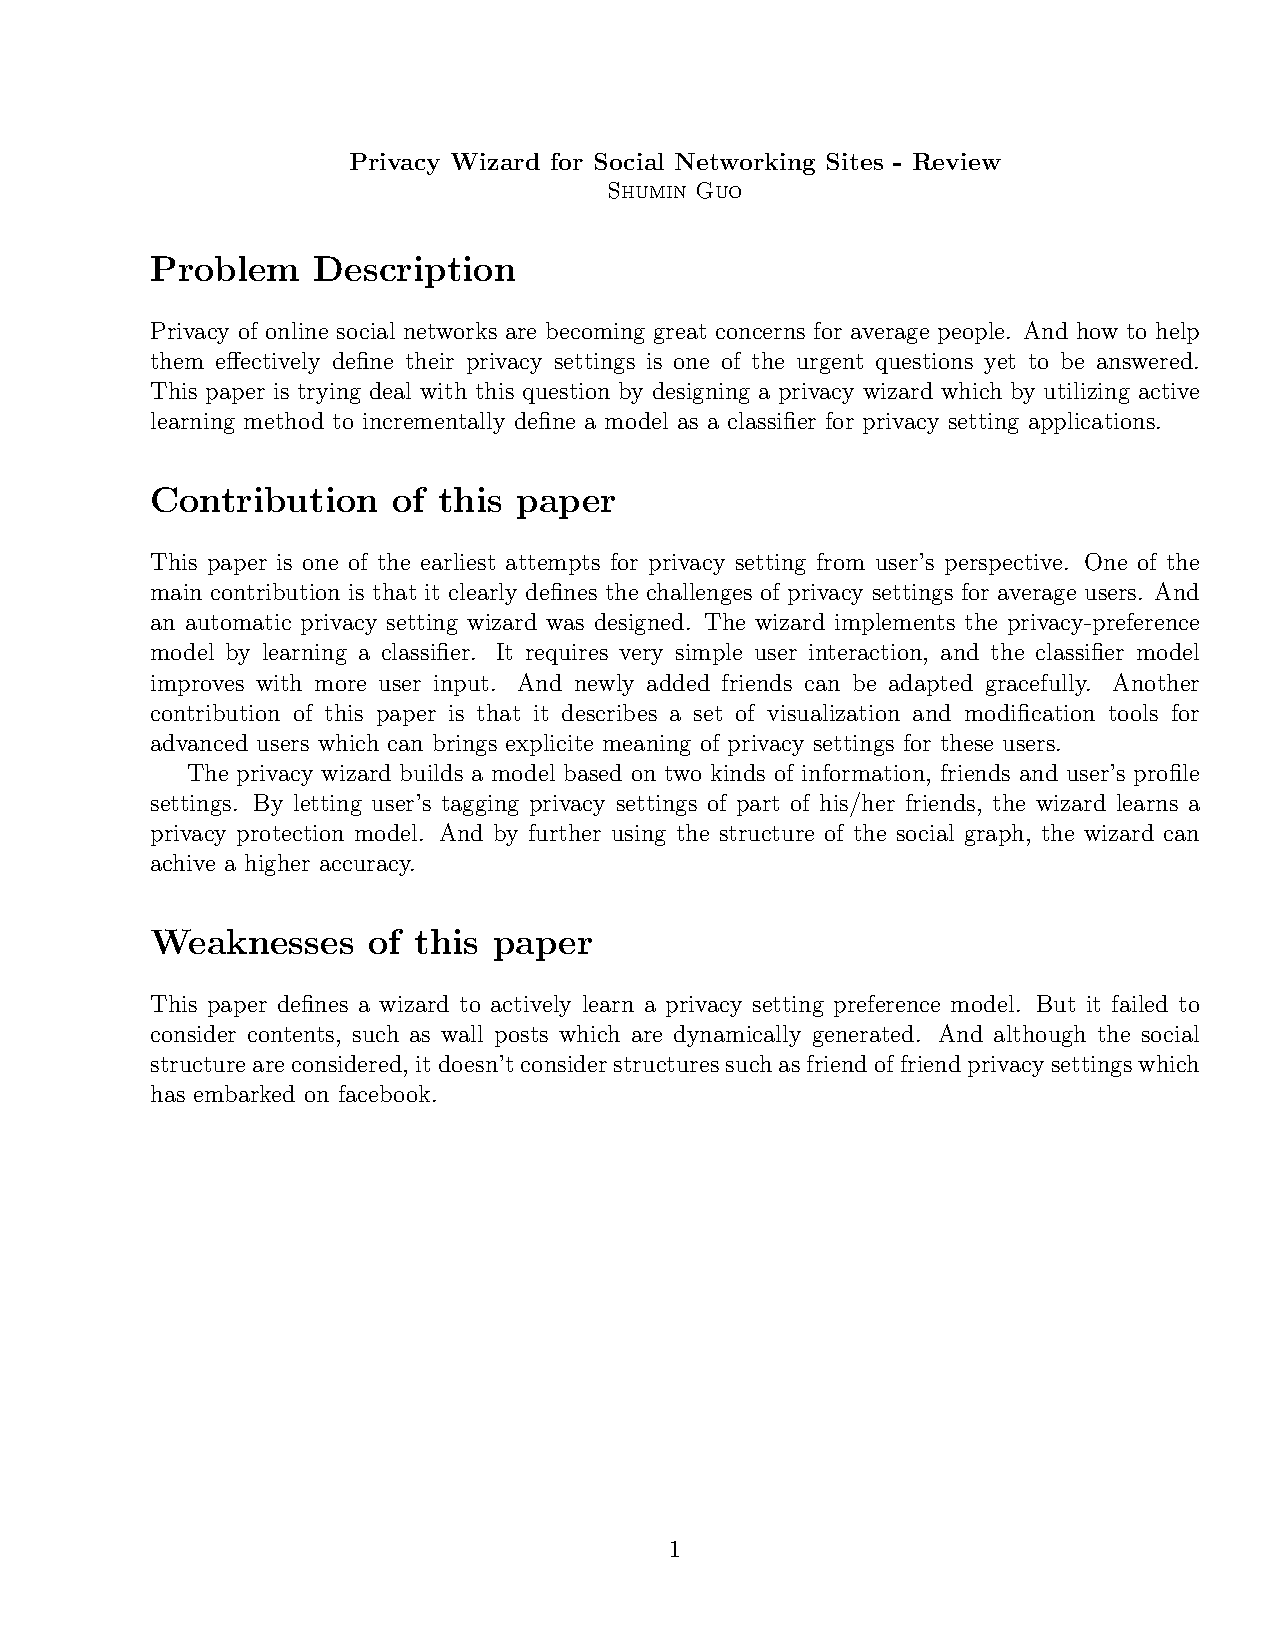
\includegraphics[scale=0.3]{wizard.pdf}%% TO BE ADDED. 
\end{figure}
\end{frame}
%
\begin{frame}[fragile] % Notice the [fragile] option %
\frametitle{Wizard Specification}
The privacy wizard solicits input from users by asking some simple
questions as shown below: 
\begin{example}[Example of wizard interaction with users]
\begin{verbatim}
Would you like to share DATE OF BIRTH with ...
Alice Adams? (Y/N)
Bob Baker?   (Y/N)
Carol Cooper?(Y/N)
...
\end{verbatim} 
\end{example} 
According to the example above, it is natural to view the
privacy-preference model as a binary classifier. This classifier can
be infered from a set of labeled training examples (such as labeled
friends) $F_{labeled}$. In this paper, the author uses feature vector
$\vec{X}$ of a friend to predict the friend's privacy label. And the
classifier can be viewed as a function of the form:
$\widehat{pref}:\vec{X}\rightarrow${allow,deny}. And the resulting
classifier can be used to predict the user's privacy preference for
unlabeled friends. 
\end{frame}

\begin{frame}[fragile]
\frametitle{Feature Selection and Extraction}
\begin{itemize}
\item Community Structure.\\
  We can extract a set of communities using $F_{labeled}$ and
  $F_{unlabeled}$. And then denote $G_1=1$ if user belongs to
  community $G_1$ and $G_1=0$ if not. 
\item Profile information of user and his friends. \\
  We can utilize the profiles, activities and other auxillary
  information(such as fans on facebook) of user's friends as
  feature 
\item Example of Extracted Features. \\
  \begin{tabular}{l*{6}{c}r}
    Name  & Age & Gender & G0 & G20  & Fan_A & Label(DOB) \\
    \hline
    Alice Adams  & 60 & F & 0 & 0 & 1 &  allow  \\
    Bob Baker    & 16 & M & 0 & 0 & 1 &  deny   \\
    Carol Cooper & 32 & M & 1 & 1 & 0 &  ?  \\
  \end{tabular}
\end{itemize}
\end{frame}
%
\begin{frame}
\frametitle{Uncertainty Sampling}
This paper utilized Uncertainty Sampling to achive the best accuracy of
the classifier with a limited amount of training data. 
\section*{Two phases of uncertainty sampling:}
\begin{itemize}
\item Sampling phase \\
  The wizard selects friends for the user to label. The rule is to
  achive highest entrophy, as according to information theory, the
  higher the entropy, the more information the message will contain.
\item Classifier Construction phase. \\
  In this phase, the wizard will use the labeled data to construct the
  classifier $(\widehat{pref})$, which is used to configure the user's
  settings. 
\end{itemize}
\end{frame}
%
\begin{frame}
\frametitle{Incremental Maintenance}
This paper considers the following two points concerned with
incremental maintenance:\\
\begin{itemize}
\item Make reasonable prediction for new users without any additional
  input from user. 
\item In case user labeled new friends, these labeled data can be
  utilized in the classifier construction process. 
\end{itemize}
With these two incremental maintenance considerations, the wizard can
not only automate the prediction of user's preference on current
friends but also the newly added friends and make the preference
classifier more and more accurate with more input (labeled
data/friends) from user. This will clearly satisfies the goal of this
paper.  
\end{frame}
%
\begin{frame}
\frametitle{A binary decision tree visulization model}
In this paper, the classifier wizard constructs a binary decision tree
and present the result to the user a visulized tree model. 
\begin{figure}
\includegraphics[scale=0.2]{tree} %%TOBE added. 
\end{figure}
\end{frame}

%
\begin{frame}
\frametitle{Evaluation}
\begin{itemize}
  \item Effectiveness.
  \item Most useful features for preference prediction. 
\end{itemize}
\end{frame}


\begin{frame}
\centerline{The End}
\end{frame}
% End of slides
\end{document}